\chapter{Diskussion der Umsetzung}
\label{chap:five}
Im folgendem Kapitel wird das Design des Prototypen besprochen und die Teilsysteme vorgestellt und skizziert wie die Teilsysteme
funktionieren. Dabei wird exemplarisch anhand von einzelnen Methoden der Klassen oder Funktionen beschrieben wie das funktioniert
Im Quellcode selber wird ausführlich jede Methode beschrieben.
\section{Design}
    \subsection{Technische Details der Implementierung}
    Das Proof-of-Concepts wurde mittels der Programmiersprache Python umgesetzt. 
    Python ist weitverbreitet, gut lesbar und gut dokumentiert. Genutzt wurde für den Datenimport und die Datenbearbeitung insbesondere die Python-Bibliothek 
    Pandas, die eine Open-Source-Bibliothek für Datenanalyse und Datenmanipulation ist. Wichtige Konzepte dieser Bibliothek sind die des Dataframes und der Series. 
    Dataframe ist eine zweidimensionale tabellarische Datenstruktur mit beschrifteten Achsen (Spalten und Reihen).
    Währenddessen eine Pandas Series ein eindimensionales Array darstellt. Auf dem Dataframe, das als sogenannter Container für
    die geladenen Daten aus csv oder xlsx-Dateien dient, können verschiedene Operationen der Datenanalyse und -manipulation erfolgen.
    Vor allem in Verbindung mit Pandas ist Python neben R und Matlab im wissenschaftlichen Kontext für Datascience-Projekte sehr beliebt.

    
    Für die Erstellung der Datenvisualisierungen wurde die Bibliothek Plotly Express genutzt. 
    Das Dashboard wurde mit dem Framework Dash entwickelt, mit welcher die Diagramme leicht eingebunden. 
    Sowohl Plotly Express als auch Dash werden von derselben Firma entwickelt. Dash baut
    auf Flask, Plotly.js und React.js auf. Das Framework ermöglicht, die Erstellung interaktiver Webapplikationen 
    in reinem Python ohne Kenntnisse von Javascript und mit wenig Wissen von HTML und CSS. \autoref{tab:Software-Requirements} zeigt einen 
    kurzen Überblick über die Versionsnummern der genutzten Programmiersprache und der Frameworks sowie deren Open-Source
    Lizenzen.
    
    \begingroup
        \setlength{\tabcolsep}{4pt} % Default value: 6pt
        \renewcommand{\arraystretch}{1.5}
        %\resizebox{\textwidth}{!}{
        \begin{table}[h]
            \centering
            \begin{adjustbox}{max width=\textwidth}
            \Huge
            \begin{tabular}{lccl}
              %\begin{tabular}{p{3cm}p{5cm}p{1cm}p{1.5cm}p{2cm}p{4cm}}
               \toprule
               \textbf{Name}             &{Version}    &\textbf{Lizenz}                        & \textbf{Webseite}\\
               \midrule     
                    Python               &3.7.9         &Open Source (PSF)                     & \url{https://docs.python.org/3.7/}\\
                    Pandas               &1.1.2         &3-Clause-BSD-License                  & \url{https://pandas.pydata.org/pandas-docs/version/1.1.2/}\\
                    Plotly Express       &0.4.0         &MIT-License                           & \url{https://plotly.com/python/}\\
                    Dash                 &1.16.3        &MIT-License                           & \url{https://dash.plotly.com/}\\


                \bottomrule
            \end{tabular}
            \end{adjustbox}
            \caption
            \label{tab:Software-Requirements}
            }
             \end{table}
        \endgroup
    
     
    \subsection{Systemarchitektur}
    
    Das System teilt sich in vier Teilsysteme auf. \autoref{tab:Teilsysteme} zeigt die vier Teilsysteme mit einer Kurzbeschreibung der Hauptaufgabe.
    Objekt-orientiert programmiert wurden nur Teile des Systems. Diese Teile sind die Bereiche des Datenimports und der Datenbearbeitung. 
    %Wohingegen die Bereiche der Darstellung mit dem Dashframework nicht mehr objektorientiert werden konnte.
    
       \begingroup
            \setlength{\tabcolsep}{4pt} % Default value: 6pt
            \renewcommand{\arraystretch}{1.5}
            %\resizebox{\textwidth}{!}{
            \begin{table}[h]
                \centering
                \begin{adjustbox}{max width=\textwidth}
                \Huge
                \begin{tabular}{lccl}
                  %\begin{tabular}{p{3cm}p{5cm}p{1cm}p{1.5cm}p{2cm}p{4cm}}
                   \toprule
                   \textbf{Teilsystem}             &{Hauptaufgabe} \\
                   \midrule     
                        Import               &Import und Transformation der Daten aus heterogenen Datenquellen.\\
                        Datenbearbeitung     &Aufbereitung der Daten für die graphische Darstellung im Dashboard.\\
                        Darstellung          &Bereitstellung der Daten und Anzeige der Daten im Dashboard.\\
                        Standardbericht      &Export ausgewählter Datenvisualisierungen und Darstellung in Berichtsform.\\

                    \bottomrule
                \end{tabular}
                \end{adjustbox}
                \caption
                \label{tab:Teilsysteme}
                }
                 \end{table}
            \endgroup
    



    

% Urls zu den als Fußnoten dazufügen.

% Herausfiltern der Datensätze zum Beispiel aus den Neuerwerbungslisten, hinter denen keine physische Entsprechung zum einen steht (mehrteilige Ressouurce auf Gesaamtitel?ebene, Datensätze Schriftenreihen)

    
    
%     grobes Bild der Systemarchitekturmit Klassen -> UML-Diagramm mit Bereichen
    
    
%     Plotly Express\\
%     Pandas\\
%     Dash\\
%     -> effizient und effektiv zu sein




%     \begin{lstlisting}[language=Python, caption=Python example]
%         import pandas as pd
%         import plotly.express as px

        
%     \end{lstlisting}

    \subsection{Teilsysteme}
    
    \textit{Import}\\
    Das Teilsystem Import ist verantwortlich für den Import der Daten im Rohformat aus vordefinierten Importverzeichnissen in vordefinierte Zielverzeichnisse. Das Ziel
    ist einerseits die Daten ohne Informationsverlust zu importieren und und andererseits diese mit notwendigen Daten anzureichern. Schließlich werden die Daten
    in ein einheitliches csv-Format umgewandelt und abgespeichert.
    % Die Daten werden jeweils in ein Pandas Dataframe geladen. Das Dataframe wird dann verschiedentlich bearbeitet, bevor es zum Schluss als csv-Datei in dem jeweiligen
    % Zielverzeichnis abgespeichert wird.
    Das Teilsystem Import besteht aus vier Klassen. Die \autoref{fig:classes import} zeigt die einzelnen Klassen mit ihren Methoden des 
    Teilsystems. Instantiiert werden die einzelnen Klassen für die jeweiligen konkreten bibliothekarischen Daten. So gibt es für Budget, Umsatz, Ausleihe usw.
    jeweils eine eigene Instanz und die für die Daten angemessenen Methoden der Klassen.
    
    \begin{figure}[H]
        \centering
            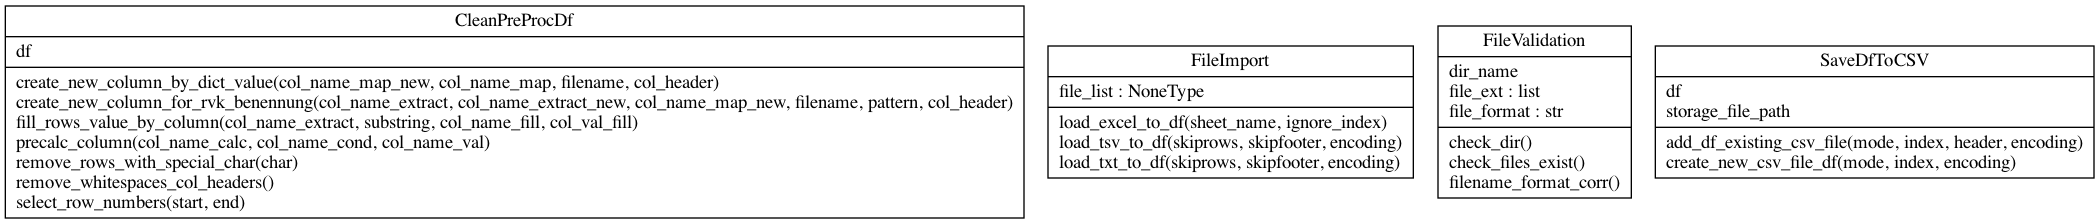
\includegraphics[width=14cm, height=2.5cm]{classes_imp}
            \caption{Klassendiagramm - Teilsystem Import}
            \label{fig:classes import}
    \end{figure}

    Die Klassen im Teilsystem Import sind auf den Daten aus fremden Quellen zugeschnitten
    (Budget Umsatz, Neuerwerbungslisten, Ausleihe (Anwendungsfall 2, 4-6)). Dennoch wurden mit ihnen auch die anderen Daten
    wie Lesesaalnutzung bearbeitet. 

    Den Ablauf des Teilsystems zeigt schematisch die \autoref{fig:flow import}.

    \begin{figure}[H]
        \centering
            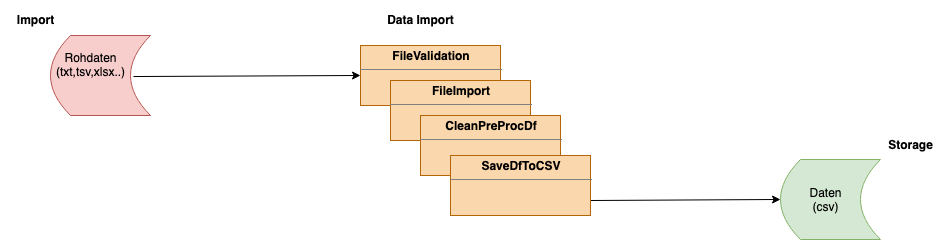
\includegraphics[width=12cm, height=2.5cm]{flow_imp}
            \caption{Datenfluss - Teilsystem Import}
            \label{fig:flow import}
    \end{figure}

    
    (1) Für den ersten Schritt sind die Klassen \texttt{FileValidation} und \texttt{FileImport} verantwortlich.
    Die Dateien werden aus einem vorher definierten lokalen Verzeichnis in ein Pandas Dataframe exportiert. 
    Dabei wird mit Methoden der Klasse \texttt{FileValidation} sichergestellt, dass sowohl das Verzeichnis als auch die Dateien existieren. 
    Des Weiteren wird sichergestellt, dass die Dateinamen einem definierten semantischen Format (z.B. YYYY\_MM\_DD) und 
    einem Format (zum Beispiel csv, xlsx) entsprechen. Da die Daten unterschiedlich aufgebaut und in unterschiedlichen Dateiformaten vorliegen 
    werden beim Import in den Dataframe jeweils verschiedene Methoden angewandt.
    Beim Ladeprozess in den Pandas Dataframe wird mit den Methoden \texttt{load\_txt\_to\_df} oder \texttt{load\_tsv\_to\_df} der Klasse \texttt{FileImport} 
    zum Zeitpunkt des Imports der Datei in den Dataframe der Dateiname extrahiert und in eine neue Spalte des Dataframe als String 
    im Datumsformat YYYY-MM-DD gespeichert. Die neu entstandene Spalte ist für die spätere Auswertung und Darstellung der Daten im Dashboard wichtig, 
    da anhand dieser Spalte die Daten nach dem Datum ausgewertet werden können.
    \footnote{Dieses Verfahren wird bei den Daten ausgeführt, die einer zusätzlichen Datumsspalte bedürfen.} 
    Verantwortlich für die Umwandlung des Dateinamens in einen String ist die in \texttt{utils.py} ausgelagerte Funktion \texttt{date\_from\_filename},
    die den Dateinamen als Parameter entgegennimmt.
    \footnote{In der Datei \texttt{utils.py} sind noch andere Funktionen als stand-alone-functions gruppiert, da diese das Objekt \texttt{self} nicht verändern.} 
    
    (2) Das geladene Pandas Dataframe wird im zweiten Schritt durch die Klasse \texttt{CleanPreProcDf} aufgenommen und durch verschiedene Methoden dieser Klasse
    manipuliert. Beispielhaft ist hier die Methode \texttt{create\_new\_column\_for\_rvk\_benennung} zu nennen, die aus der Spalte der Signatur 
    der Neuerwerbungen die Hauptklassen der \textit{\acrlong{RVK}} extrahiert. Dieser Methode liegt eine csv-Datei
    der \textit{\acrshort{RVK}} zu Grunde, die mit einem Skript aus der \textit{\acrshort{RVK}}-XML-Datei entstanden ist. Ergänzt wurde diese noch um eigene Hauptklassen 
    der Institutsbibliothek, die an die in der Form an die \textit{\acrshort{RVK}} angelehnt sind. Des Weiteren gibt es in der Klasse Methoden die für die Entfernung von Rows
    mit bestimmten syntaktischen Zeichen wie einem Bindestrich verantwortlich oder die unnötige Leerzeichen Spaltenköpfen löschen und mit einem Leerzeichen ersetzen.
     
    (3) Nachdem Transformationsprozess wird das veränderte Pandas Dataframe als csv-Datei in einem vorher definierten Zielordner gespeichert. 
    Verantwortlich ist dabei die Klasse \texttt{SaveDFToCSV} mit den zwei Methoden \texttt{add\_df\_existing\_csv\_file create\_new\_csv\_file\_df}. 
    Die je nach dem mit dem Dataframe eine neue csv-Datei kreiren oder an eine bereits vorhandene csv-Datei den Dataframe anhängen.
    
    \begin{figure}[h]
        \centering
            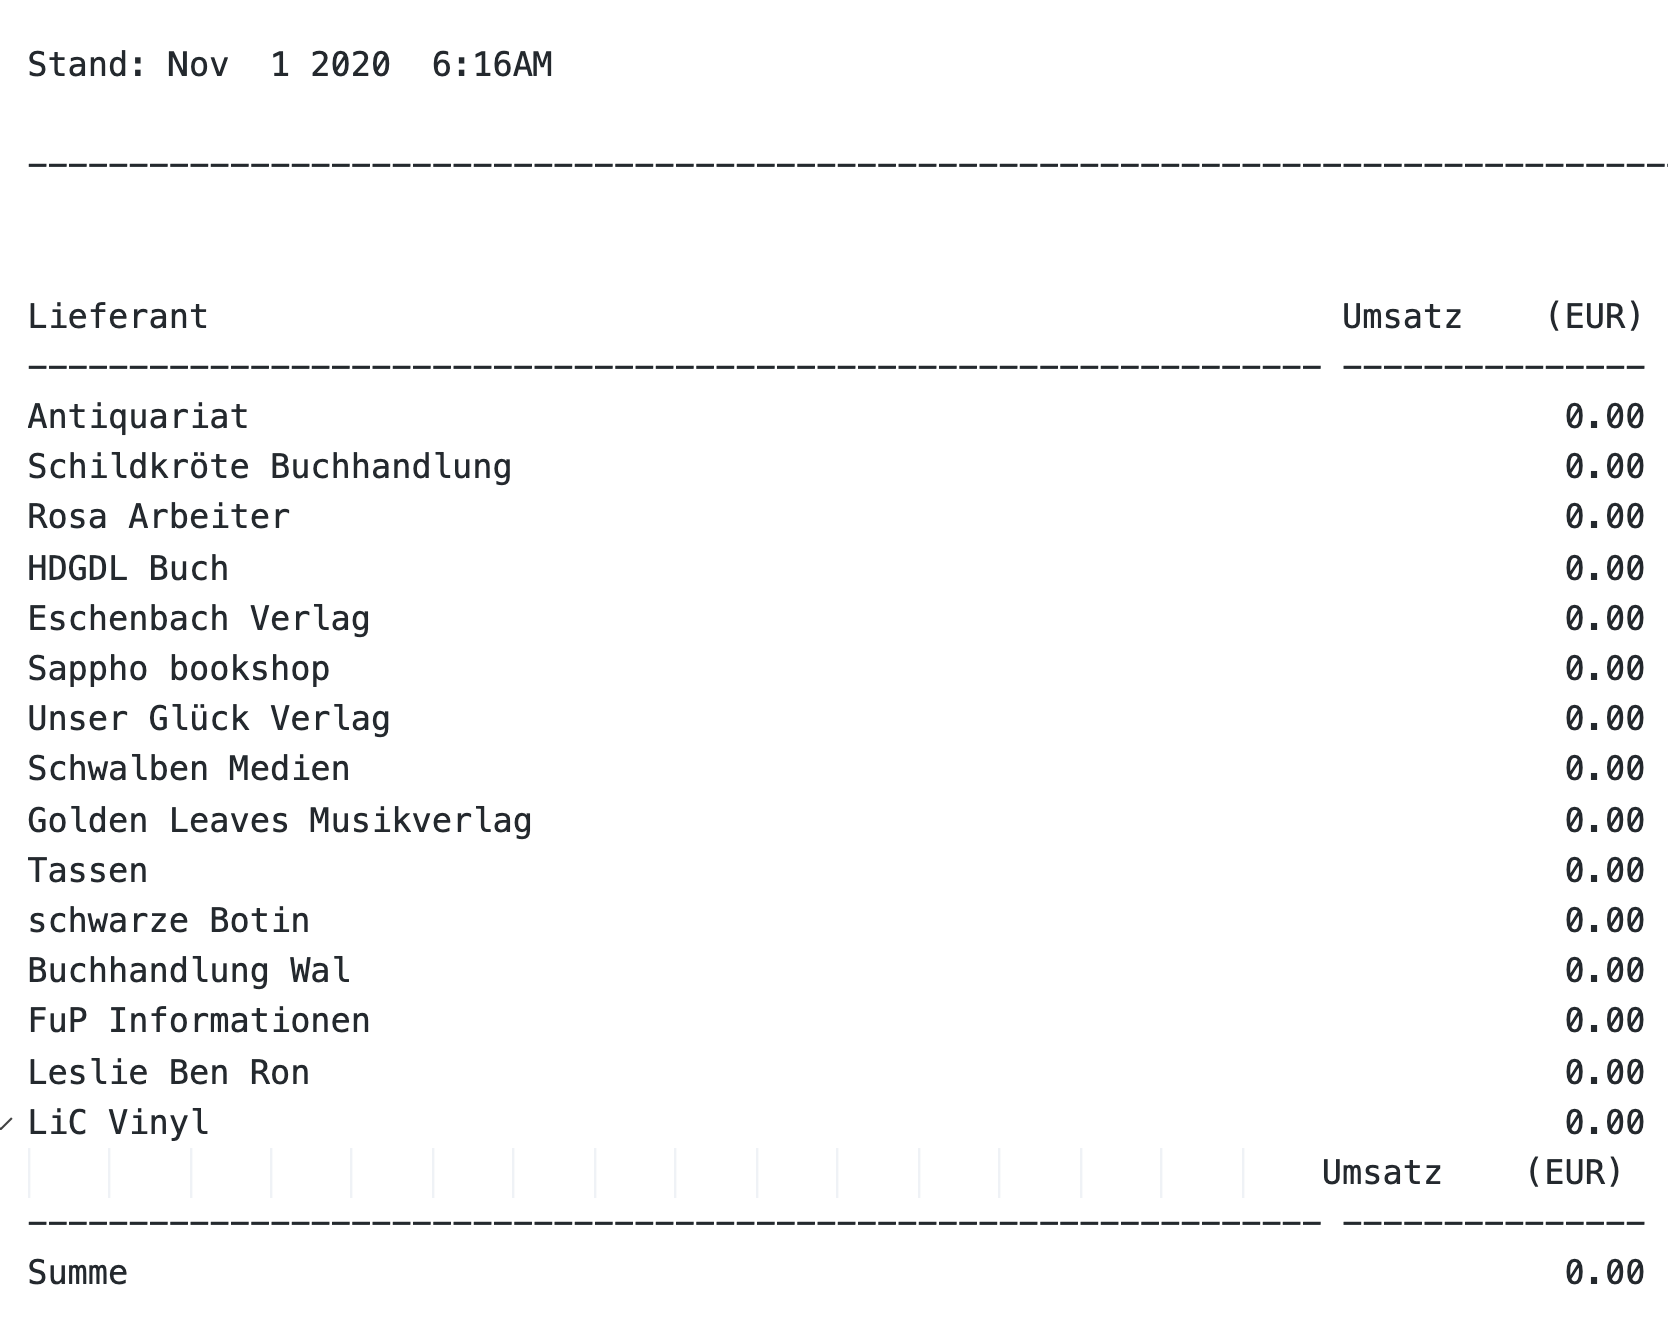
\includegraphics[width=6.5cm, height=7.0cm]{umsatzuebersicht_mtl}
            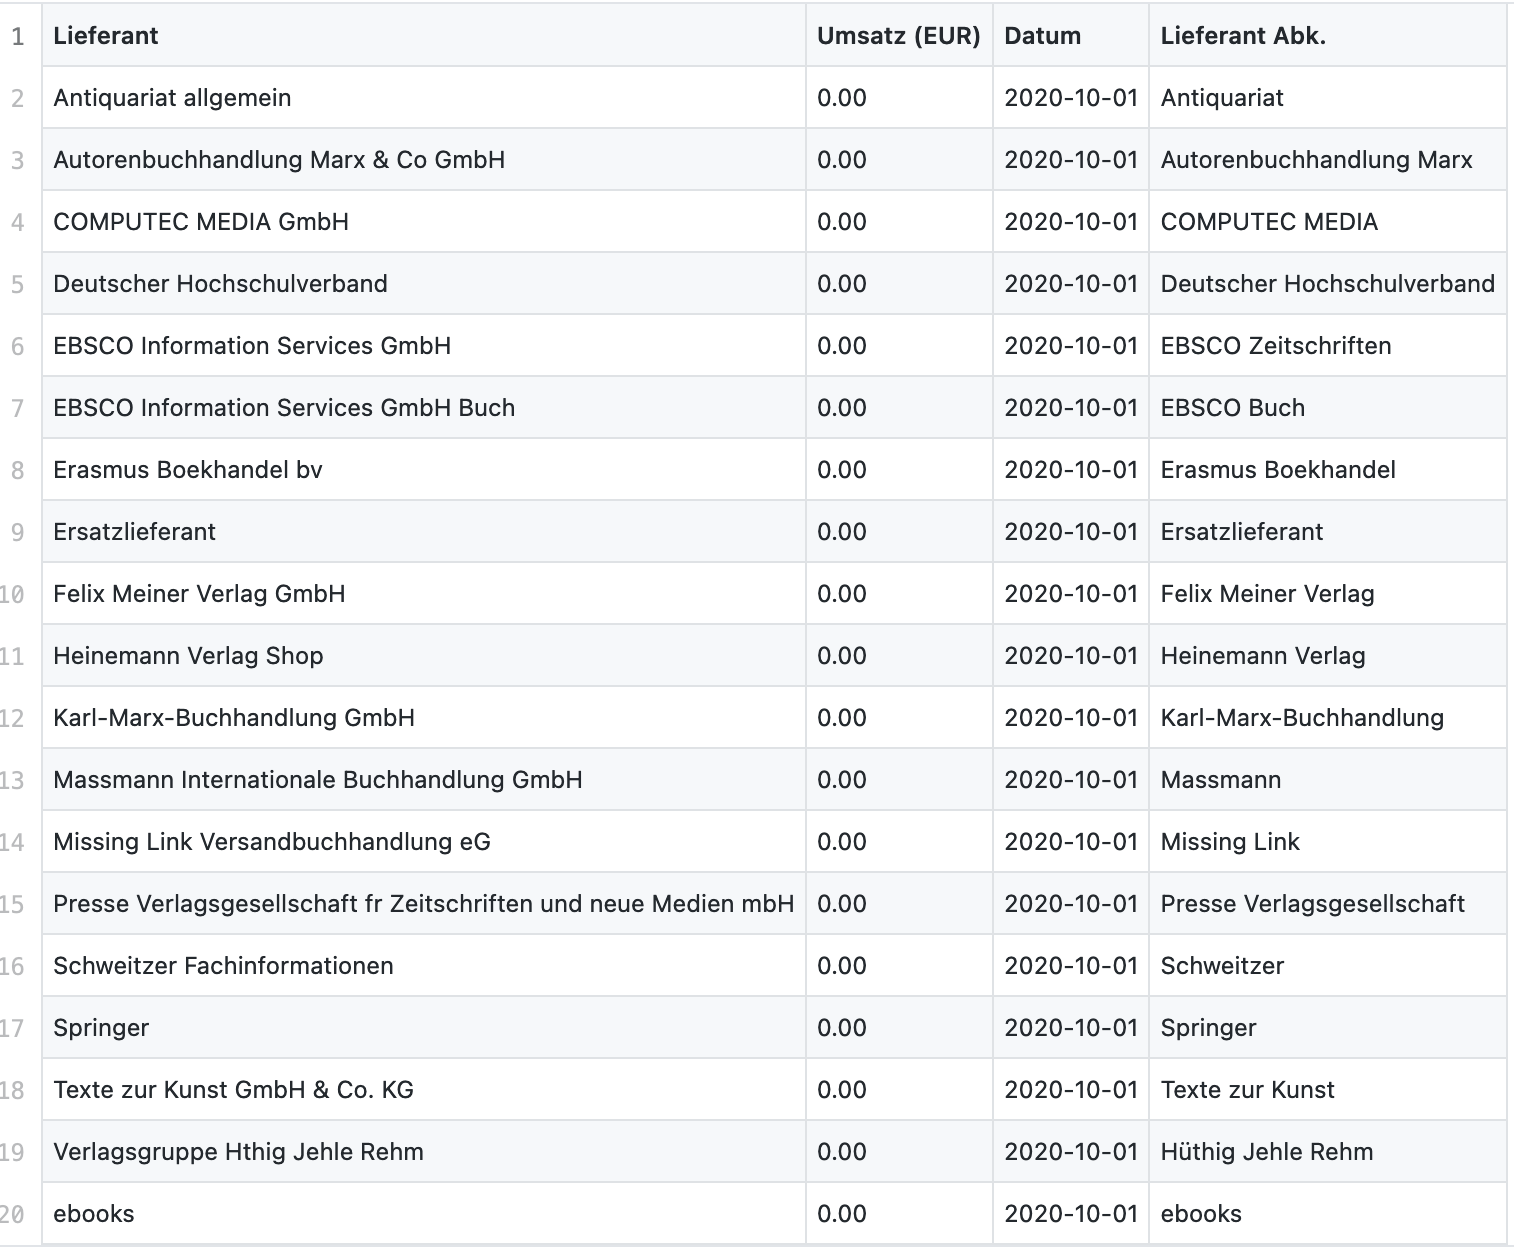
\includegraphics[width=6.5cm, height=7.0cm]{umsatz_csv_bsp}
            \caption{Monatliche Budget- und Umsatzübersicht}
            \label{fig:umsatzuebersicht_csv}
    \end{figure}
    

    Am Beispiel der Umsatzdaten 
    

\section{Implementierung}

  

    \subsection{Umgesetzte Anforderungen}
    Folgende Must-Anforderungen wurden erfüllt.
    R1, R2, R3, R4, R5, R7
    F1, F4, F5, F12
    NF5, NF6, 
    \subsection{Funktionsweise}
    Das Layout des Dashboards besteht aus drei Tabs. Diese wurden nach den Bereichen der Bibliothek aufgeteilt. Diese Aufteilung erschien als sinnvoll,
    da auf grafische Oberfläche nicht überladen werden sollte.
    Nach dem der Webserver gestartet wurde, landet man im Tab1 und bekommt die dort verankerten Inhalte zu sehen.
    Tabs sind als Reiter oben auf der Webseite angesiedelt.
    Drauf klicken und man gelangt auf den Inhalt desa Tabs (Seite)
    
    Fast allen Diagrammen wohnt inne, dass man aus der Legende auswählen kann welche Elemente angezeigt bzw. nicht angezeigt werden sollen.
    mitunter auch hover elemente, wenn über die einzelnen Balken oder Linien mit der Maus gefahre 
    
    Tab1 - Umsatz und Budget
    
    Bild Tab1
    Was ist dargestellt:
    
    zwei Diagramme mit 
        Anzeige des Gesamtumsatz nach Jahren und nach Lieferanten ->  horizontalestapeltes Balkendiagramm
        umsatzstärkste Lieferanten (Top 7) Verteilung in Prozent (Kreisdiagramm)
        
    zwei Diagramme mit interaktiver Auswahl eines Lieferanten über Dropdownmenü
        Anzeige des Gesamtumsatzes nach Jahren für de ausgewählten Lieferanten (Liniendiagramm)
        Anzeige des Umsatzes pro Monat für das laufende Jahr (Balkendiagramm)
    
    zwei Diagramme mit
        Anzeige des Gesamtbudgets nach Jahren und nach Kostenstellen 
        Anzeige kostenintesive (Top 7) Kostenstellen
        
    
    vier Karten mit
        Zahl des Gesamtumsatzes
        Zahl des Umsatzes im Jahr
        Zahl des Umsatzes im laufenden Jahrs für den einzelnen Lieferanten (gekoppelt mit Dropdown-Auswahl)
        Durchschnittlicher Umsatz des Lieferanten (gekoppelt mit Dropdown-Auswahl)
    
    
    
    
    
    Tab2 - Lesesaal und Ausleihe
    
    Bild Tab2
    
    zwei Diagramme mit
        Anzeige der Nutzer:innen nach Jahren und nach Service-Zeiten (gruppiertes Balkendiagramm)
        Anzeige der Nutzer:innen nach Monaten und nach Service-Zeiten für das laufende Jahr.
        
     ein Diagramm mit
        Anzeige der Ausleihanzahl nach Jahren (horizontales Balkendiagramm)
    
    Tab3 - Bestand
    
    Bild Tab3

    
     



\section{Bewertung}
